% Options for packages loaded elsewhere
\PassOptionsToPackage{unicode}{hyperref}
\PassOptionsToPackage{hyphens}{url}
%
\documentclass[
]{article}
\usepackage{amsmath,amssymb}
\usepackage{iftex}
\ifPDFTeX
  \usepackage[T1]{fontenc}
  \usepackage[utf8]{inputenc}
  \usepackage{textcomp} % provide euro and other symbols
\else % if luatex or xetex
  \usepackage{unicode-math} % this also loads fontspec
  \defaultfontfeatures{Scale=MatchLowercase}
  \defaultfontfeatures[\rmfamily]{Ligatures=TeX,Scale=1}
\fi
\usepackage{lmodern}
\ifPDFTeX\else
  % xetex/luatex font selection
\fi
% Use upquote if available, for straight quotes in verbatim environments
\IfFileExists{upquote.sty}{\usepackage{upquote}}{}
\IfFileExists{microtype.sty}{% use microtype if available
  \usepackage[]{microtype}
  \UseMicrotypeSet[protrusion]{basicmath} % disable protrusion for tt fonts
}{}
\makeatletter
\@ifundefined{KOMAClassName}{% if non-KOMA class
  \IfFileExists{parskip.sty}{%
    \usepackage{parskip}
  }{% else
    \setlength{\parindent}{0pt}
    \setlength{\parskip}{6pt plus 2pt minus 1pt}}
}{% if KOMA class
  \KOMAoptions{parskip=half}}
\makeatother
\usepackage{xcolor}
\usepackage[left=2cm,right=2cm,top=2.5cm,bottom=2.5cm]{geometry}
\usepackage{longtable,booktabs,array}
\usepackage{calc} % for calculating minipage widths
% Correct order of tables after \paragraph or \subparagraph
\usepackage{etoolbox}
\makeatletter
\patchcmd\longtable{\par}{\if@noskipsec\mbox{}\fi\par}{}{}
\makeatother
% Allow footnotes in longtable head/foot
\IfFileExists{footnotehyper.sty}{\usepackage{footnotehyper}}{\usepackage{footnote}}
\makesavenoteenv{longtable}
\usepackage{graphicx}
\makeatletter
\def\maxwidth{\ifdim\Gin@nat@width>\linewidth\linewidth\else\Gin@nat@width\fi}
\def\maxheight{\ifdim\Gin@nat@height>\textheight\textheight\else\Gin@nat@height\fi}
\makeatother
% Scale images if necessary, so that they will not overflow the page
% margins by default, and it is still possible to overwrite the defaults
% using explicit options in \includegraphics[width, height, ...]{}
\setkeys{Gin}{width=\maxwidth,height=\maxheight,keepaspectratio}
% Set default figure placement to htbp
\makeatletter
\def\fps@figure{htbp}
\makeatother
\setlength{\emergencystretch}{3em} % prevent overfull lines
\providecommand{\tightlist}{%
  \setlength{\itemsep}{0pt}\setlength{\parskip}{0pt}}
\setcounter{secnumdepth}{5}
\ifLuaTeX
\usepackage[bidi=basic]{babel}
\else
\usepackage[bidi=default]{babel}
\fi
\babelprovide[main,import]{french}
% get rid of language-specific shorthands (see #6817):
\let\LanguageShortHands\languageshorthands
\def\languageshorthands#1{}
\usepackage{fancyhdr}
\pagestyle{fancy}
\fancyhf{} % Efface les en-têtes et pieds de page par défaut
\fancyhead[L]{EL MAZZOUJI Wahel, GILLET Louison} % À gauche
\fancyhead[C]{} % Au centre (laisser vide si non utilisé)
\fancyhead[R]{M1 - SSD} % À droite
\fancyfoot[C]{\thepage} % Numéro de page au centre du pied de page
\ifLuaTeX
  \usepackage{selnolig}  % disable illegal ligatures
\fi
\IfFileExists{bookmark.sty}{\usepackage{bookmark}}{\usepackage{hyperref}}
\IfFileExists{xurl.sty}{\usepackage{xurl}}{} % add URL line breaks if available
\urlstyle{same}
\hypersetup{
  pdftitle={Trouver un titre évocateur et moins formel},
  pdfauthor={EL MAZZOUJI Wahel; GILLET Louison},
  pdflang={true},
  hidelinks,
  pdfcreator={LaTeX via pandoc}}

\title{Trouver un titre évocateur et moins formel}
\author{EL MAZZOUJI Wahel \and GILLET Louison}
\date{2024/2025}

\begin{document}
\maketitle

\begin{figure}[h!]
    \centering
    
\includegraphics[width=0.5\linewidth]{ssd.png}
\end{figure}

\newpage

\tableofcontents

\newpage

\hypertarget{introduction}{%
\section{INTRODUCTION}\label{introduction}}

Dans le cadre de notre étude, nous avons accès à un jeu de données riche
qui examine la diversité de 27 espèces d'arbres au sein de 1000
parcelles forestières. Cette analyse vise à explorer la variabilité des
densités de peuplement de ces espèces dans le contexte particulier de la
forêt du bassin du Congo. Le jeu de données se compose de 30 variables
quantitatives, dont les principales incluent le comptage des individus
pour chaque espèce, la superficie de chaque parcelle ainsi que deux
variables supplémentaires relatives au type forestier et au type
géologique. À cela s'ajoute une variable qualitative, identifiée par un
``code'', qui permet d'apporter des informations contextuelles sur
chaque parcelle. Cette étude permettra d'éclairer les dynamiques
écologiques en jeu et d'approfondir notre compréhension des interactions
entre les espèces arborées et leur environnement.

\hypertarget{donnees-et-but}{%
\section{DONNEES ET BUT}\label{donnees-et-but}}

\hypertarget{partie-1}{%
\section{PARTIE 1}\label{partie-1}}

\hypertarget{densituxe9s}{%
\subsection{Densités}\label{densituxe9s}}

\hypertarget{densituxe9-de-peuplement}{%
\subsubsection{Densité de peuplement}\label{densituxe9-de-peuplement}}

Nous cherchons à calculer la densité de peuplement de chaque espèce par
unité de surface. Pour chaque parcelle, la densité est donnée par :

\[
D_{ij} = \frac{N_{ij}}{S_{j}}
\]

où \(D_{ij}\) est la densité pour l'espèce \(i\) dans la parcelle \(j\),
\(N_{ij}\) est le nombre d'individus de l'espèce \(i\) dans la parcelle
\(j\) et \(S_{j}\) est la surface de la parcelle \(j\).

Nous utilisons des densités plutôt que des comptages car cela permet de
normaliser les données par rapport à la taille de la parcelle, ce qui
rend les comparaisons entre les parcelles équitables.

\begin{longtable}[]{@{}rrrrrrr@{}}
\caption{Extrait du tableau des densités de peuplement}\tabularnewline
\toprule\noalign{}
gen1 & gen2 & gen3 & gen4 & gen5 & gen6 & gen7 \\
\midrule\noalign{}
\endfirsthead
\toprule\noalign{}
gen1 & gen2 & gen3 & gen4 & gen5 & gen6 & gen7 \\
\midrule\noalign{}
\endhead
\bottomrule\noalign{}
\endlastfoot
0.0000000 & 0.0000000 & 0.0 & 0 & 0.0000000 & 0.4000000 & 0.0000000 \\
0.6000000 & 0.0000000 & 0.2 & 0 & 0.1333333 & 0.1333333 & 0.0666667 \\
0.5142857 & 0.0000000 & 0.0 & 0 & 0.0571429 & 0.0000000 & 0.1714286 \\
0.0000000 & 0.1951220 & 0.0 & 0 & 0.4390244 & 0.0487805 & 0.5365854 \\
0.0952381 & 0.0952381 & 0.0 & 0 & 0.0000000 & 0.0000000 & 0.3809524 \\
\end{longtable}

\hypertarget{densituxe9-centruxe9e-ruxe9duite}{%
\subsubsection{Densité
centrée-réduite}\label{densituxe9-centruxe9e-ruxe9duite}}

Nous devons centrer et réduire les variables quantitatives pour mieux
comparer celles qui décrivent les différentes densités. Nous allons
utiliser la formule suivante pour le centrage et la réduction :

\[
Z_{ij} = \frac{D_{ij} - \bar{D_{j}}}{s_{j}}
\]

où \(\bar{D_{j}}\) est la moyenne pour la variable \(j\) et \(s_{j}\)
l'écart-type de la variable quantitative \(j\).

\begin{longtable}[]{@{}
  >{\raggedleft\arraybackslash}p{(\columnwidth - 12\tabcolsep) * \real{0.1429}}
  >{\raggedleft\arraybackslash}p{(\columnwidth - 12\tabcolsep) * \real{0.1429}}
  >{\raggedleft\arraybackslash}p{(\columnwidth - 12\tabcolsep) * \real{0.1429}}
  >{\raggedleft\arraybackslash}p{(\columnwidth - 12\tabcolsep) * \real{0.1429}}
  >{\raggedleft\arraybackslash}p{(\columnwidth - 12\tabcolsep) * \real{0.1429}}
  >{\raggedleft\arraybackslash}p{(\columnwidth - 12\tabcolsep) * \real{0.1429}}
  >{\raggedleft\arraybackslash}p{(\columnwidth - 12\tabcolsep) * \real{0.1429}}@{}}
\caption{Extrait du tableau des densités
centrées-réduites}\tabularnewline
\toprule\noalign{}
\begin{minipage}[b]{\linewidth}\raggedleft
gen1
\end{minipage} & \begin{minipage}[b]{\linewidth}\raggedleft
gen2
\end{minipage} & \begin{minipage}[b]{\linewidth}\raggedleft
gen3
\end{minipage} & \begin{minipage}[b]{\linewidth}\raggedleft
gen4
\end{minipage} & \begin{minipage}[b]{\linewidth}\raggedleft
gen5
\end{minipage} & \begin{minipage}[b]{\linewidth}\raggedleft
gen6
\end{minipage} & \begin{minipage}[b]{\linewidth}\raggedleft
gen7
\end{minipage} \\
\midrule\noalign{}
\endfirsthead
\toprule\noalign{}
\begin{minipage}[b]{\linewidth}\raggedleft
gen1
\end{minipage} & \begin{minipage}[b]{\linewidth}\raggedleft
gen2
\end{minipage} & \begin{minipage}[b]{\linewidth}\raggedleft
gen3
\end{minipage} & \begin{minipage}[b]{\linewidth}\raggedleft
gen4
\end{minipage} & \begin{minipage}[b]{\linewidth}\raggedleft
gen5
\end{minipage} & \begin{minipage}[b]{\linewidth}\raggedleft
gen6
\end{minipage} & \begin{minipage}[b]{\linewidth}\raggedleft
gen7
\end{minipage} \\
\midrule\noalign{}
\endhead
\bottomrule\noalign{}
\endlastfoot
-0.9525149 & -0.4458588 & -0.3833563 & -0.3454747 & -0.4504654 &
1.6585968 & -0.4433017 \\
0.7194413 & -0.4458588 & 0.5368654 & -0.3454747 & 0.4379021 & 0.1954714
& -0.2791772 \\
0.4805904 & -0.4458588 & -0.3833563 & -0.3454747 & -0.0697365 &
-0.5360913 & -0.0212673 \\
-0.9525149 & 0.1536780 & -0.3833563 & -0.3454747 & 2.4746469 &
-0.2684465 & 0.8777003 \\
-0.6871251 & -0.1532277 & -0.3833563 & -0.3454747 & -0.4504654 &
-0.5360913 & 0.4945525 \\
\end{longtable}

\hypertarget{barycentre-et-inertie}{%
\subsection{Barycentre et inertie}\label{barycentre-et-inertie}}

\hypertarget{barycentre-uxe0-lorigine}{%
\subsubsection{Barycentre à l'origine}\label{barycentre-uxe0-lorigine}}

Considérons que nous avons un ensemble de données \(X\) composé de \(n\)
observations et \(p\) variables. Après le centrage et la réduction, la
matrice transformée \(X'\) est définie par :

\[
X'_{ij} = \frac{D_{ij} - \bar{D_{j}}}{s_{j}}
\]

Le barycentre de \(X\) est donné par la moyenne de chaque colonne de
\(X\). Calculons cette moyenne pour la variable \(j\) :

\[
\bar{D_{j}} = \frac{1}{n} \sum_{i=1}^{n} X'_{ij} = \frac{1}{n} \sum_{i=1}^{n} \left( \frac{D_{ij} - \bar{D_{j}}}{s_{j}} \right) 
= \frac{1}{s_{j}} \left( \frac{1}{n} \sum_{i=1}^{n} D_{ij} \right) - \frac{\bar{D_{j}}}{s_{j}} = 0
\]

Ainsi, le barycentre de chaque variable dans \(X'\) est égal à zéro.

\hypertarget{inertie-totale}{%
\subsubsection{Inertie totale}\label{inertie-totale}}

Considérons à nouveau la matrice de données \(X\). Après centrage et
réduction, chaque élément de la matrice transformée \(X'\) est défini
par :

\[
X'_{ij} = \frac{D_{ij} - \bar{D_{j}}}{s_{j}}
\]

L'inertie de l'ensemble des points \(X'\) par rapport à leur barycentre
\(y_M\) est définie par :

\[
I_{Y,W} = \sum_{i=1}^{n} w_{i} \|X_{i} - y_M\|^{2}
\]

où \(y_M = \frac{\sum_{i=1}^{n} w_{i} X_{i}}{\sum_{i=1}^{n} w_{i}}\) est
le barycentre pondéré. Pour les données centrées-réduites, chaque
\(X'_{i}\) est déjà centré, donc le barycentre \(y_M = 0\). Par
conséquent, la formule de l'inertie se simplifie à :

\[
I_{Y,W} = \sum_{i=1}^{n} w_{i} \|X'_{i}\|^{2}
\]

Si tous les poids \(w_{i}\) sont égaux (par exemple,
\(w_{i} = \frac{1}{n}\)), alors l'inertie devient :

\[
I_{Y,W} = \frac{1}{n} \sum_{i=1}^{n} \|X'_{i}\|^{2}
\]

Comme chaque \(X'_{i}\) est une observation centrée-réduite et que la
variance de chaque variable est 1, nous avons :

\[
\|X'_{i}\|^{2} = \sum_{j=1}^{p} (X'_{ij})^{2} = p
\]

Ainsi, l'inertie totale est :

\[
I_{Y,W} = \frac{1}{n} \sum_{i=1}^{n} p = p
\]

Ce qui montre que l'inertie totale du nuage des données
centrées-réduites est égale au nombre de variables \(p\).

\hypertarget{types-forestiers}{%
\subsection{Types forestiers}\label{types-forestiers}}

\hypertarget{inertie-inter-types}{%
\subsubsection{Inertie inter-types}\label{inertie-inter-types}}

L'inertie inter-types est calculée par :

\[
I_{inter-types} = \sum_{k=1}^{p} w_{k} \cdot n_{k}^{2}
\]

où \(p\) est le nombre de types forestiers, \(w_{k}\) est le poids du
type forestier \(k\) et \(n_{k}\) est la norme euclidienne carrée pour
ce type.

\hypertarget{coefficient-de-duxe9termination-ruxb2}{%
\subsubsection{Coefficient de détermination
R²}\label{coefficient-de-duxe9termination-ruxb2}}

Le coefficient de détermination \(R^2\) est donné par :

\[
R^2 = \frac{I_{inter-types}}{I_{total}}
\]

Ce qui représente la proportion de variance expliquée par les types
forestiers dans la variabilité des densités de peuplement.

\hypertarget{pourcentage-dinformation}{%
\subsubsection{Pourcentage
d'information}\label{pourcentage-dinformation}}

\hypertarget{liens-entre-espuxe8ces-et-types-forestiers}{%
\subsection{Liens entre espèces et types
forestiers}\label{liens-entre-espuxe8ces-et-types-forestiers}}

Nous devons vérifier que le \(R^2\) de la partition est égal à la
moyenne des \(R^2\) des espèces. Pour cela, nous calculons le \(R^2\)
pour chaque espèce \(i\) :

\[
R^2_{i} = \frac{I_{inter,i}}{I_{total,i}}
\]

Puis, nous comparons avec :

\[
R^2_{partition} = \frac{1}{m} \sum_{i=1}^{m} R^2_{i}
\]

où \(m\) est le nombre d'espèces.

\begin{figure}[ht!]

{\centering 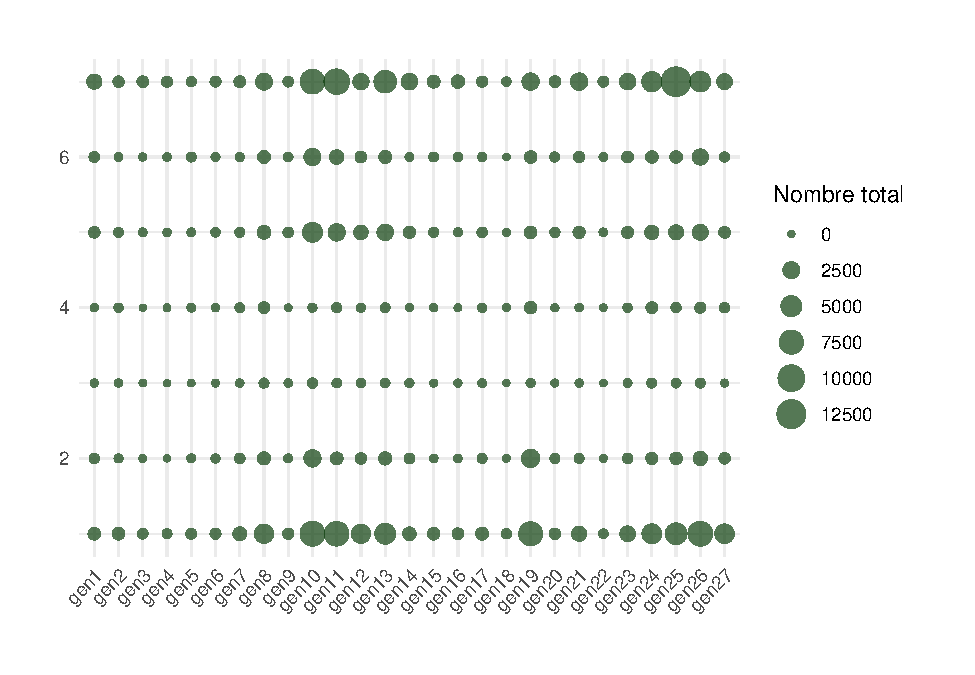
\includegraphics{EL_MAZZOUJI_Wahel_GILLET_Louison_ADM_DM1_files/figure-latex/especes_forest-1} 

}

\caption{Répartition des espèces d'arbres par type forestier}\label{fig:especes_forest}
\end{figure}

\newpage

\hypertarget{partie-2}{%
\section{PARTIE 2}\label{partie-2}}

Nous savons que l'espace \(Y\) peut être décomposé de la manière
suivante : \[
\langle Y \rangle = \langle 1 \rangle + \langle Y_{\text{centré}} \rangle
\] où \(\langle 1 \rangle\) est le sous-espace vectoriel engendré par le
vecteur constant \(\mathbf{1}\), et
\(\langle Y_{\text{centré}} \rangle\) représente le sous-espace
vectoriel engendré par \(Y\) une fois centré.

La projection \(\Pi_Y x^j\) peut donc être décomposée comme suit : \[
\Pi_Y x^j = \Pi_1 x^j + \Pi_{Y_{\text{centré}}} x^j
\] où \(\Pi_1 x^j\) est la projection de \(x^j\) sur le vecteur
constant, et \(\Pi_{Y_{\text{centré}}} x^j\) est la projection de
\(x^j\) sur l'espace engendré par les colonnes de \(Y_{\text{centré}}\).

Cependant, la projection sur le vecteur constant, \(\Pi_1 x^j\), est
égale à zéro, car \(x^j\) est une variable centrée. Autrement dit,
lorsque nous projetons \(x^j\) sur le vecteur constant, nous obtenons :
\[
\Pi_1 x^j = 0
\] En substituant cette relation dans l'équation précédente, nous
obtenons : \[
\Pi_Y x^j = 0 + \Pi_{Y_{\text{centré}}} x^j
\] d'où il s'ensuit que : \[
\Pi_Y x^j = \Pi_{Y_{\text{centré}}} x^j
\]

Ainsi, nous avons montré que, pour tout \(j\), la projection de \(x^j\)
sur \(Y\) est égale à la projection de \(x^j\) sur
\(Y_{\text{centré}}\).\newline Le fait que ces deux projections soient
égales signifie que la projection sur cet espace (lié aux types
forestiers) est la même qu'elle soit centrée ou non, car les types
forestiers sont des variables qualitatives représentées par des
indicatrices. Le centrage ne change donc pas le résultat.

On a : \[
\| \Pi_Y x^j \|_W^2 = \langle \Pi_Y x^j, \Pi_Y x^j \rangle_W
\] La projection de \(x^j\) sur \(Y\) est donnée par : \[
\Pi_Y x^j = \sum_{q=1}^{Q} w^q (\overline{x}^q - \overline{x})
\] où \(\overline{x}^q\) est la moyenne pondérée de \(x^j\) pour le type
forestier \(q\), et \(\overline{x}\) est la moyenne globale.

Statistiquement, \(\| \Pi_Y x^j \|_W^2\) représente la variance
inter-groupes de \(x^j\), c'est-à-dire la part de la variance totale de
\(x^j\) qui est expliquée par les types forestiers : \[
\| \Pi_Y x^j \|_W^2 = \sum_{q=1}^{Q} w^q (\overline{x^q} - \overline{x})^2
\]

Cette expression mesure la part de la variabilité de \(x^j\) expliquée
par la partition en types forestiers.

\hypertarget{programmation-et-calcul-de-pi_y-pi_x_j-puis-de-texttrpi_x_j-pi_y}{%
\subsection{\texorpdfstring{Programmation et calcul de \(\Pi_Y\),
\(\Pi_{x_j}\) puis de
\(\text{tr}(\Pi_{x_j} \Pi_Y)\)}{Programmation et calcul de \textbackslash Pi\_Y, \textbackslash Pi\_\{x\_j\} puis de \textbackslash text\{tr\}(\textbackslash Pi\_\{x\_j\} \textbackslash Pi\_Y)}}\label{programmation-et-calcul-de-pi_y-pi_x_j-puis-de-texttrpi_x_j-pi_y}}

\hypertarget{calcul-de-pi_y}{%
\subsubsection{\texorpdfstring{Calcul de
\(\Pi_Y\)}{Calcul de \textbackslash Pi\_Y}}\label{calcul-de-pi_y}}

Le projecteur \(\Pi_Y\) est défini comme le projecteur sur l'espace
généré par les colonnes de la matrice \(Y\). Mathématiquement, il est
formulé comme suit :

\[
   \Pi_Y = Y \left( Y' W Y \right)^{-1} Y' W
   \]

\hypertarget{calcul-de-pi_x_j}{%
\subsubsection{\texorpdfstring{Calcul de
\(\Pi_{x_j}\)}{Calcul de \textbackslash Pi\_\{x\_j\}}}\label{calcul-de-pi_x_j}}

De la même manière, nous avons :

\[
   \Pi_{x_j} = {x_j} \left( {x_j}' W {x_j} \right)^{-1} {x_j}' W
   \]

\hypertarget{calcul-de-texttrpi_x_j-pi_y}{%
\subsubsection{\texorpdfstring{Calcul de
\(\text{tr}(\Pi_{x_j} \Pi_Y)\)}{Calcul de \textbackslash text\{tr\}(\textbackslash Pi\_\{x\_j\} \textbackslash Pi\_Y)}}\label{calcul-de-texttrpi_x_j-pi_y}}

Pour chaque vecteur \(x_j\), le calcul de \(\text{tr}(\Pi_{x_j} \Pi_Y)\)
implique la projection de \(x_j\) dans l'espace défini par \(Y\). Cette
opération nous permet d'évaluer la quantité de variabilité dans \(x_j\)
qui est expliquée par la classification en types forestiers.
Ainsi,\[ \text{tr}(\Pi_{x_j} \Pi_Y) = R^2 \] où \(R^2\) représente la
proportion de variance expliquée par les types forestiers dans la
variabilité des densités de peuplement.

\hypertarget{calcul-de-texttrr-pi_y-et-interpruxe9tation-statistique}{%
\subsection{\texorpdfstring{Calcul de \(\text{tr}(R \Pi_Y)\) et
interprétation
statistique}{Calcul de \textbackslash text\{tr\}(R \textbackslash Pi\_Y) et interprétation statistique}}\label{calcul-de-texttrr-pi_y-et-interpruxe9tation-statistique}}

On note \[ R = X M X' W \].

Alors \(\text{tr}(R \Pi_Y)\) représente la somme des variances
expliquées par la partition en types forestiers, comme représenté par
\(Y\), sur l'ensemble des variables contenues dans la matrice \(X\).
Cette valeur constitue une mesure de l'inertie inter-types forestiers et
fournit une indication globale de la quantité d'information expliquée
par la classification des types forestiers sur l'ensemble des variables
analysées.

\hypertarget{calcul-de-texttrpi_x_j-pi_z-texttrr-pi_z-et-interpruxe9tation-statistique}{%
\subsection{\texorpdfstring{Calcul de \(\text{tr}(\Pi_{x_j} \Pi_Z)\),
\(\text{tr}(R \Pi_Z)\) et interprétation
statistique}{Calcul de \textbackslash text\{tr\}(\textbackslash Pi\_\{x\_j\} \textbackslash Pi\_Z), \textbackslash text\{tr\}(R \textbackslash Pi\_Z) et interprétation statistique}}\label{calcul-de-texttrpi_x_j-pi_z-texttrr-pi_z-et-interpruxe9tation-statistique}}

Le projecteur \(\Pi_Z\) est défini sur l'espace des indicatrices de
sols, représentées par la matrice \(Z\). Le calcul de
\(\text{tr}(\Pi_{x_j} \Pi_Z)\) permet d'évaluer combien de la
variabilité de \(x_j\) est expliquée par la partition en types de sols.
La formule correspondante est :

\[
\text{tr}(\Pi_{x_j} \Pi_Z)
\]

En parallèle, \(\text{tr}(R \Pi_Z)\) quantifie la somme des variances
expliquées par la partition en types de sols sur toutes les variables
dans \(X\). Cette valeur constitue une mesure de l'inertie inter-sols et
fournit une indication globale de la quantité d'information expliquée
par la classification des sols sur l'ensemble des variables analysées.

\hypertarget{conclusion}{%
\section{CONCLUSION}\label{conclusion}}

Cette analyse nous a permis de mieux comprendre les dynamiques de
peuplement forestier dans la forêt du bassin du Congo. En intégrant des
approches statistiques robustes, nous avons pu quantifier la variabilité
des espèces et leur répartition en fonction des types forestiers. Les
résultats de cette étude fourniront des bases solides pour des
recherches futures et des actions de conservation.

\end{document}
